\subsection{Semi-leptonic final state}
\label{sec:oneL} 

Events fall into the Semi-leptonic (1L) analysis category if they contain at least one pre-selected diphoton pair, and contain exactly one electron or muon passing the selection criteria described in Section \ref{sec:Phase_II_ObjectSel}. This final state is expected to be the most sensitive of the three $WW\gamma\gamma$ channels due to the combination of a relatively large $W\rightarrow qq$ branching ratio, and the presence of a highly energy lepton from the $W\rightarrow \ell\nu$ decay. 

In order to maximize the sensitivity of this final state, two multiclass DNNs are trained to separate the di-Higgs signal from the resonant single Higgs boson background and continuum background where the di-Higgs processes are labelled as \textit{HH}, single Higgs backgrounds as \textit{H} and all other background samples as continuum background.

% (HH $\rightarrow$ 2$\gamma 2ql\nu$, HH $\rightarrow$ $2\gamma 2\tau$, HH $\rightarrow 2 \gamma 2l2\nu$) 

During training, each class has a weight applied which scales the event loss such that the effective importance's of each of the three classes are equalized. This ensures that the network focuses on categorising all classes with an equal importance. 

Two multiclass DNNs are trained, one which trains on one half of simulation events, and a second which trains on the other half of simulation events. This separation on simulation datasets allows one to apply the training performed with “even” events on the “odd” data set, and vice versa, to avoid any training bias.

The simulation sample variables used as inputs for the DNN trainings include the kinematic variables such as $p_T$, $\eta$, $\phi$ and energy values of photons, jets, electrons and muons. For photons, $p_T$ and energy values are scaled by the diphoton mass in order to avoid the creation of an artificial resonance among continuum background processes. Additionally, the jet multiplicity, missing transverse energy and the invariant mass of the leading and subleading jets are utilized in the trainings. 

The multiclass DNN outputs three DNN scores, one for each class, but only the HH output DNN score is used in the analysis. The HH DNN score distribution is shown in Figure \ref{fig:oneL_perf}. 

\begin{figure}[!htb]
    \centering
    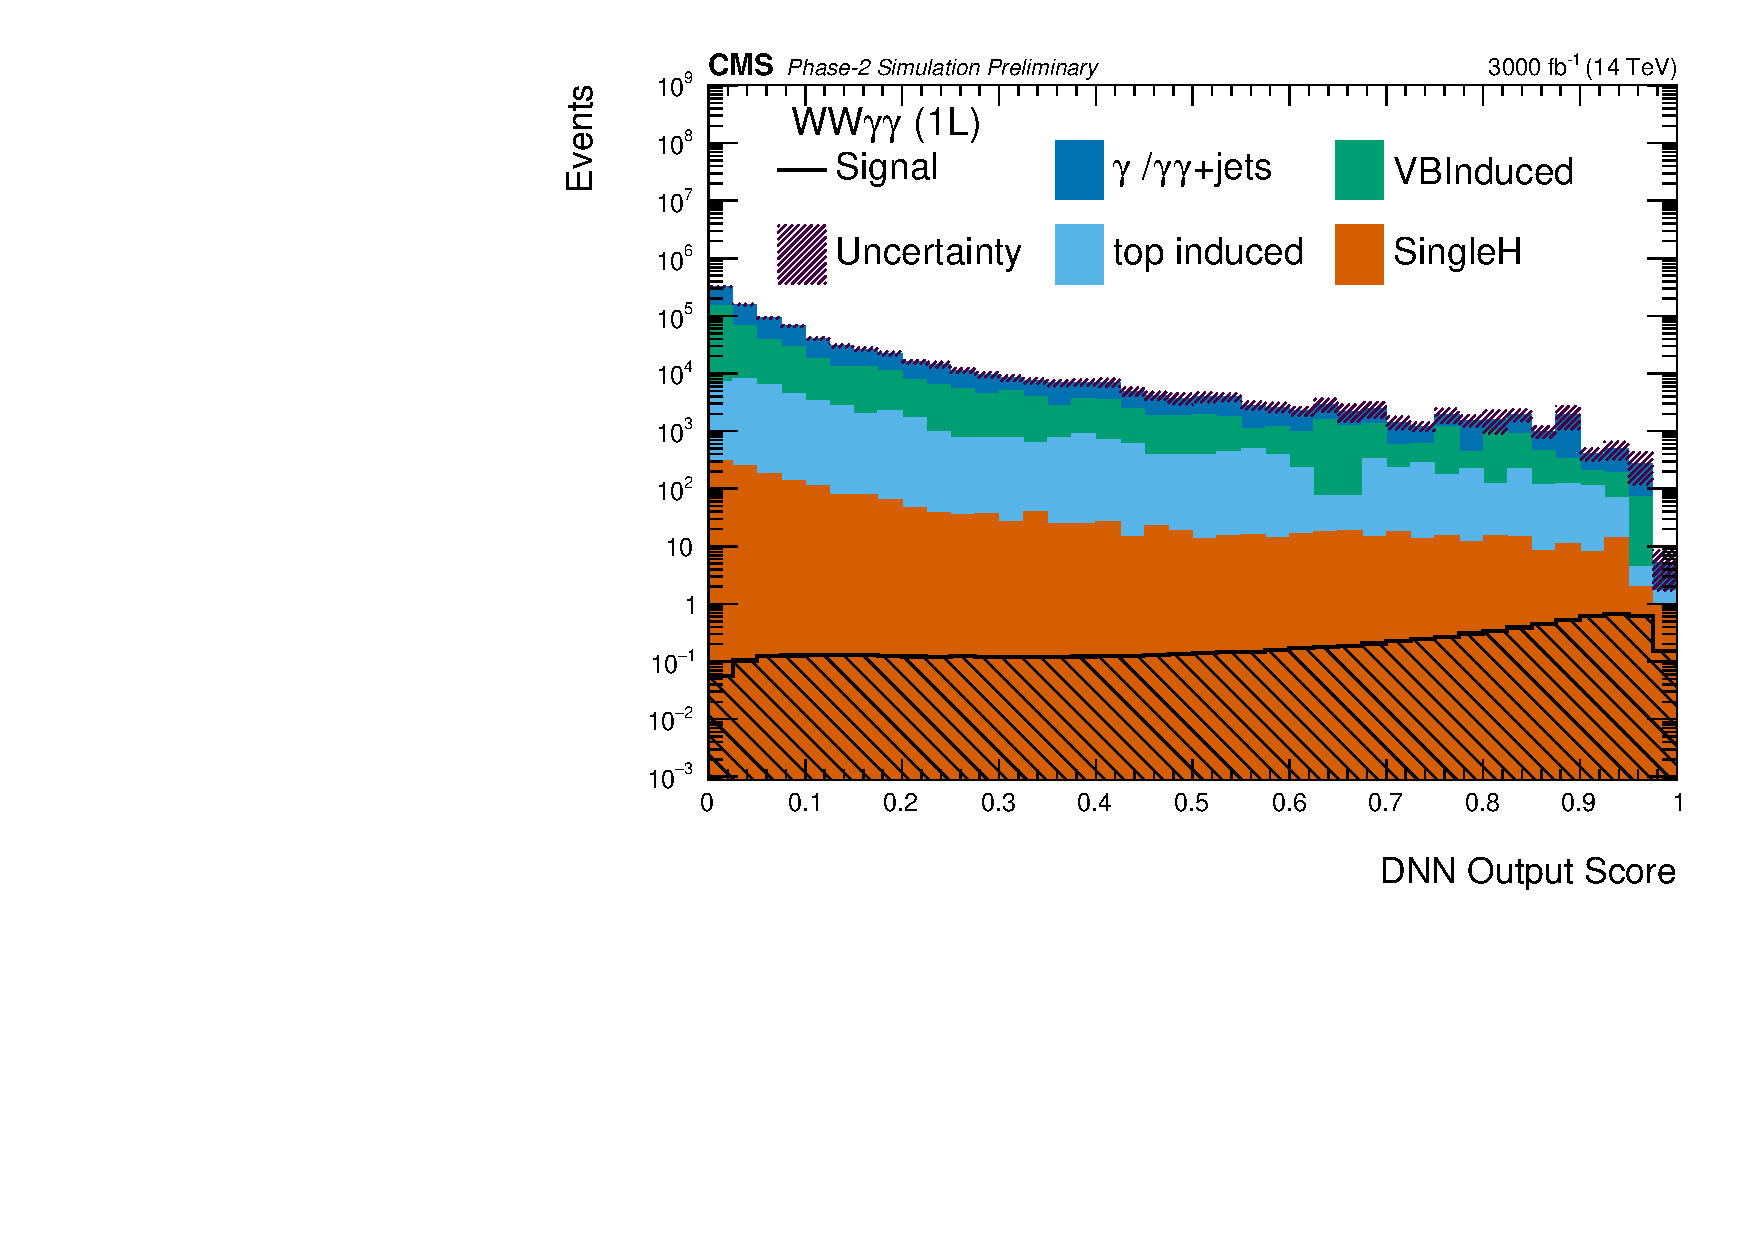
\includegraphics[width=0.75\textwidth]{Sections/Phase_II_HH/images/DNN/DNN_Score_WW_logy.pdf}
    \caption{Semi-leptonic DNN output score distribution.}
    \label{fig:oneL_perf}
\end{figure}

In order to further optimize the analysis sensitivity, events are partitioned into four categories making use of the \textit{HH} node output score. The category boundaries are chosen such that the expected significance is maximized, and are shown in Table \ref{tab:OneLcats}.

\begin{table}[!htb]
  \centering
  \begin{tabular}{ll}
    \hline 
    Categories & Definition\\
    \hline 
    Category 1  & 0.1 $<$ DNN score $<$ 0.6 \\
    Category 2  & 0.6 $<$ DNN score $<$ 0.8 \\
    Category 3  & 0.8 $<$ DNN score $<$ 0.92 \\
    Category 4  & DNN score $>$ 0.92 \\
    \hline
   \end{tabular}
    \caption{
      Semi-leptonic final state DNN score categories.
    }
    \label{tab:OneLcats}
\end{table}

This categorization leads to an improved combined significance as opposed to using a single category, as multiple regions with reasonable signal sensitivities can be combined. Category four is the category with the highest signal purity and significance.  


